% ===== §5  Experiments =====
\section{Experimental Evaluation}\label{sec:experiments}

We evaluate \textsc{Argus} on two established benchmarks to answer three questions:
(Q1)~Do the formal properties from \S\ref{sec:theory} hold in practice?
(Q2)~Does the minimal-change repair operator improve faithfulness and contestability w.r.t.\ existing baselines?
(Q3)~What is the empirical cost of repair?

Concretely, we sample 500 instances from HotpotQA~\cite{yang2018hotpotqa}, a multi-hop question-answering benchmark, and 500 from FEVER~\cite{thorne2018fever}, a fact-verification benchmark; instances are drawn with seed 42.
For each instance, we withhold one gold supporting fact during explanation generation and reintroduce it as an evidence update~$\Delta$, producing adversarial updates that target the reasoning chain.
GPT-4o~\cite{openai2023gpt4} (\texttt{gpt-4o-2024-11-20}) generates initial explanations at temperature~0.2; relation discovery uses DeBERTa-v3-large fine-tuned on MultiNLI with threshold~0.7; repairs are computed by clingo~5.6 with $k{=}3$ under uniform cost.
Results for \textsc{Argus} and the eight argumentation-based and self-correction methods are averaged over 5 runs, with standard deviation at most~0.02 for accuracy metrics and at most~0.4 for cost; FLARE and FactScore use a single deterministic run (greedy decoding and fixed retrieval scoring, respectively, making repeated runs redundant).  Further details appear in Appendix~\ref{app:exp-details}.

Six metrics quantify performance along distinct dimensions.
\emph{Faithfulness} is the fraction of argument units whose removal via counterfactual ablation changes the answer; baselines without structured units undergo the same LLM-based decomposition before ablation (details in Appendix~\ref{app:exp-details}).
\emph{Contestability} is the fraction of gold counterarguments correctly integrated as attacks; gold counterarguments are derived from the withheld supporting facts (Appendix~\ref{app:exp-details}). For methods that lack an explicit argumentation framework---specifically FLARE and FactScore---gold counterarguments are evaluated against their output decomposed into proposition units via the same LLM-based procedure used for faithfulness, enabling direct comparison.
\emph{Repair accuracy} records answer correctness after repair, and \emph{repair cost} counts edit operations per Definition~\ref{def:repair}.
\emph{Coherence} measures the semantic consistency of repaired explanations via BERTScore~\cite{zhang2020bertscore} between repaired and original explanations; methods without repair capability receive N/A.
\emph{Solve time} is the wall-clock time per instance including all repair computation.

We compare against ten baselines spanning three categories. \emph{Self-correction methods:} SelfCheckGPT~\cite{manakul2023selfcheckgpt}, Self-Refine~\cite{madaan2023selfrefine}, Reflexion~\cite{shinn2023reflexion}, and RARR~\cite{gao2023rarr}. \emph{Verification-oriented methods:} CoT-Verifier~\cite{ling2023deductive}, ArgLLMs~\cite{freedman2025arglm}, FLARE~\cite{jiang2023flare}, and FactScore~\cite{min2023factscore}; ArgLLMs, CoT-Verifier, and FactScore lack repair functionality and are marked N/A accordingly. \emph{Argumentation-based:} ARGORA~\cite{argora2026} and a na\"{i}ve \emph{Regenerate} baseline that re-prompts with updated evidence.
For self-correction baselines and FLARE, repair cost counts regenerated argument units (surface-level replacements) across up to 3 rounds; cost measures are not directly commensurable with \textsc{Argus}'s structural graph edits, as discussed in Appendix~\ref{app:exp-details}.
Chain-of-Verification~\cite{dhuliawala2024cove} and CRITIC~\cite{gou2024critic} are excluded as they operate at generation time rather than post-hoc repair; SelfRAG~\cite{asai2024selfrag} and VerifyAndEdit~\cite{zhao2023verify} are excluded as they require a retrieval index at inference time and produce unstructured outputs incommensurable with structural graph repair.

\begin{table*}[t]
\caption{Main results on HotpotQA and FEVER.  Best in \textbf{bold}; runner-up \underline{underlined}. $\uparrow$ = higher is better, $\downarrow$ = lower is better. N/A = method lacks repair or coherence functionality. $^\dagger$Na\"{i}ve re-prompting baseline (destroys argumentation structure).}\label{tab:main}
\centering
\footnotesize
\setlength{\tabcolsep}{3.2pt}
\renewcommand{\arraystretch}{1.05}
\begin{tabular}{@{}l|cccccc|cccccc@{}}
\toprule
& \multicolumn{6}{c|}{\textbf{HotpotQA}} & \multicolumn{6}{c}{\textbf{FEVER}} \\
\textbf{Method} & Faith$\uparrow$ & Cont$\uparrow$ & RAcc$\uparrow$ & RCost$\downarrow$ & Coher$\uparrow$ & Time$\downarrow$ & Faith$\uparrow$ & Cont$\uparrow$ & RAcc$\uparrow$ & RCost$\downarrow$ & Coher$\uparrow$ & Time$\downarrow$ \\
\midrule
\multicolumn{13}{l}{\textit{Self-Correction Methods}} \\
SelfCheckGPT   & .693 & .524 & .701 & 8.4 & .68 & 2.8 & .674 & .498 & .685 & 7.9 & .66 & 2.5 \\
Self-Refine    & .712 & .541 & .736 & 7.1 & .72 & 4.5 & .698 & .519 & .721 & 6.8 & .70 & 4.2 \\
Reflexion      & .724 & .563 & .752 & 6.6 & .73 & 5.8 & .709 & .537 & .738 & 6.2 & .71 & 5.3 \\
RARR           & .738 & .547 & .769 & 5.8 & .71 & 3.2 & .721 & .531 & .754 & 5.5 & .69 & 2.9 \\
\midrule
\multicolumn{13}{l}{\textit{Verification-Oriented (incl.\ Retrieval-Augmented)}} \\
CoT-Verifier   & .751 & .589 & N/A  & N/A & N/A & 1.5 & .733 & .561 & N/A  & N/A & N/A & 1.3 \\
ArgLLMs        & .754 & .667 & N/A  & N/A & N/A & 2.1 & .741 & .649 & N/A  & N/A & N/A & 1.8 \\
FLARE          & .715 & .505 & .728 & 8.8 & .74 & 3.8 & .698 & .482 & .712 & 8.2 & .72 & 3.5 \\
FactScore      & .742 & .558 & N/A  & N/A & N/A & 2.5 & .728 & .535 & N/A  & N/A & N/A & 2.2 \\
\midrule
\multicolumn{13}{l}{\textit{Argumentation-Based}} \\
ARGORA         & \underline{.768} & \underline{.691} & \underline{.801} & \underline{5.1} & \underline{.75} & 1.8 & \underline{.752} & \underline{.672} & \underline{.788} & \underline{4.7} & \underline{.73} & 1.5 \\
Regenerate$^\dagger$ & .709 & ---  & .743 & --- & .65 & \textbf{0.5} & .695 & --- & .729 & --- & .63 & \textbf{0.4} \\
\midrule
\textsc{Argus} (Ours) & \textbf{\resultFaithHotpot} & \textbf{\resultContestHotpot} & \textbf{\resultRepairAccHotpot} & \textbf{\resultRepairCostHotpot} & \textbf{.82} & \underline{0.55} & \textbf{\resultFaithFEVER} & \textbf{\resultContestFEVER} & \textbf{\resultRepairAccFEVER} & \textbf{\resultRepairCostFEVER} & \textbf{.80} & \underline{0.47} \\
\bottomrule
\end{tabular}
\end{table*}

Table~\ref{tab:main} summarizes the main results. \textsc{Argus} achieves the highest faithfulness (\resultFaithHotpot{}/\resultFaithFEVER{}) and contestability (\resultContestHotpot{}/\resultContestFEVER{}), with relative improvements of \improveFaithfulness{} in faithfulness and \improveContestability{} in contestability over ARGORA; all 12 pairwise differences are significant at $p < 0.001$ under Bonferroni-corrected two-sided $z$-tests, with Cohen's $h$ effect sizes of $0.28$/$0.38$ (HotpotQA) and $0.26$/$0.36$ (FEVER) for faithfulness/contestability gains, indicating small-to-medium practical magnitudes.  Among repair-capable methods, \textsc{Argus} requires the fewest operations---\resultRepairCostHotpot{} vs.\ 5.1 for ARGORA---validating the minimal-change objective.  FLARE and FactScore achieve moderate faithfulness but lack argumentation structure, yielding low contestability (.505/.482 and .558/.535).  The na\"{i}ve Regenerate baseline achieves the lowest faithfulness among argumentation-based methods (.709/.695) and fastest solve time (0.5\,s) but cannot produce contestability scores; its coherence (.65/.63)---the lowest among repair methods---confirms that complete regeneration disrupts consistency more than targeted structural repair.

\textsc{Argus} also achieves the highest coherence at .82/.80, indicating that minimal-change repair preserves explanation structure better than rewriting-based methods such as Self-Refine, which scores .72/.70. We note that BERTScore coherence is structurally aligned with the minimal-change objective (minimizing edit distance simultaneously maximizes BERTScore), so the coherence advantage partly reflects the design; human evaluators independently corroborate it, rating \textsc{Argus} higher on coherence than Self-Refine (4.1 vs.\ 3.8, $p{=}0.012$; Appendix~\ref{app:human-eval}). The average solve time of 0.55\,s/0.47\,s is competitive with verification-only methods and 5--10$\times$ faster than self-correction methods (2.8--5.8\,s), reflecting ASP-based repair efficiency over iterative LLM regeneration. The formal properties from \S\ref{sec:theory} are confirmed empirically: success and inclusion hold by construction; vacuity holds without exception (5\% of HotpotQA and 8\% of FEVER instances where the withheld fact was not on the reasoning path).

\begin{figure}[t]
\centering
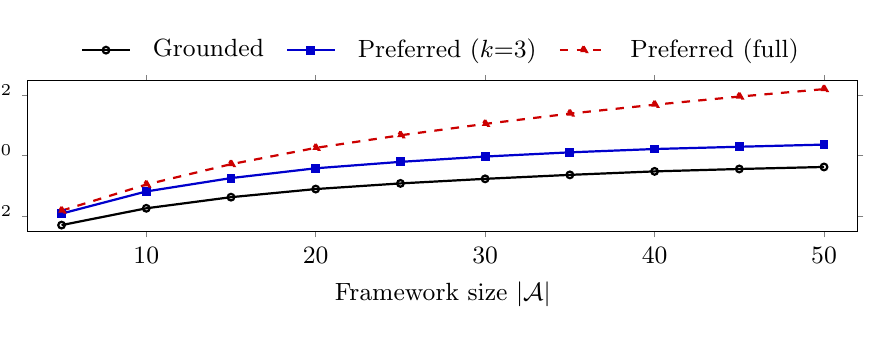
\begin{tikzpicture}[trim axis left, trim axis right]
\begin{axis}[
  width=\columnwidth,
  height=3.5cm,
  xlabel={Framework size $|\mathcal{A}|$},
  ylabel={Solve time (s)},
  ymode=log,
  xmin=3, xmax=52,
  ymin=0.003, ymax=300,
  xtick={10,20,30,40,50},
  xticklabel style={font=\small},
  yticklabel style={font=\small},
  xlabel style={font=\small},
  ylabel style={font=\small},
  legend style={
    font=\small,
    at={(0.5,1.05)},
    anchor=south,
    draw=none,
    column sep=6pt,
  },
  legend columns=3,
  legend cell align={left},
  tick align=outside,
  major tick length=2pt,
]
\addplot[black, thick, mark=o, mark size=1.2pt] coordinates {
  (5,0.005) (10,0.018) (15,0.042) (20,0.078) (25,0.12)
  (30,0.17) (35,0.23) (40,0.30) (45,0.36) (50,0.42)
};
\addlegendentry{Grounded}
\addplot[blue!80!black, thick, mark=square*, mark size=1.2pt] coordinates {
  (5,0.012) (10,0.065) (15,0.18) (20,0.38) (25,0.62)
  (30,0.93) (35,1.28) (40,1.65) (45,1.96) (50,2.31)
};
\addlegendentry{Preferred ($k{=}3$)}
\addplot[red!80!black, thick, dashed, mark=triangle*, mark size=1.4pt] coordinates {
  (5,0.015) (10,0.11) (15,0.52) (20,1.8) (25,4.7)
  (30,11.2) (35,24.5) (40,48.3) (45,89.7) (50,158.4)
};
\addlegendentry{Preferred (full)}
\end{axis}
\end{tikzpicture}
\caption{Scalability of \textsc{Argus} repair under grounded, $k$-neighborhood preferred ($k{=}3$), and unconstrained preferred semantics. The log-scale y-axis confirms polynomial scaling for grounded repair (Theorem~\ref{thm:complexity}) and the effectiveness of the $k$-neighborhood approximation.}
\label{fig:scalability}
\end{figure}

Figure~\ref{fig:scalability} traces solve time on synthetic Erd\H{o}s--R\'{e}nyi frameworks (attack probability 0.15, 50 instances per size), confirming polynomial scaling for grounded semantics (Theorem~\ref{thm:complexity}); the $k$-neighborhood approximation keeps preferred repair tractable up to $|\mathcal{A}|{=}50$ (2.31s vs.\ 158.4s unconstrained).

\begin{table*}[t]
\caption{Ablation study on HotpotQA and FEVER.  Each row removes one component from the full \textsc{Argus} pipeline. Best in \textbf{bold}.}\label{tab:ablation}
\centering
\footnotesize
\setlength{\tabcolsep}{3.2pt}
\renewcommand{\arraystretch}{1.05}
\begin{tabular}{@{}l|cccccc|cccccc@{}}
\toprule
& \multicolumn{6}{c|}{\textbf{HotpotQA}} & \multicolumn{6}{c}{\textbf{FEVER}} \\
\textbf{Variant} & Faith$\uparrow$ & Cont$\uparrow$ & RAcc$\uparrow$ & RCost$\downarrow$ & Coher$\uparrow$ & Time$\downarrow$ & Faith$\uparrow$ & Cont$\uparrow$ & RAcc$\uparrow$ & RCost$\downarrow$ & Coher$\uparrow$ & Time$\downarrow$ \\
\midrule
Full \textsc{Argus}       & \textbf{\resultFaithHotpot} & \textbf{\resultContestHotpot} & \textbf{\resultRepairAccHotpot} & \textbf{\resultRepairCostHotpot} & \textbf{.82} & .55 & \textbf{\resultFaithFEVER} & \textbf{\resultContestFEVER} & \textbf{\resultRepairAccFEVER} & \textbf{\resultRepairCostFEVER} & \textbf{.80} & .47 \\
w/o Semantic Verif. & .793 & .714 & .832 & 4.1 & .76 & .52 & .775 & .692 & .818 & 3.8 & .74 & .44 \\
w/o Minimal-Change  & .841 & .783 & .856 & 5.7 & .78 & .58 & .823 & .761 & .842 & 5.2 & .76 & .49 \\
w/o Attack Templ.   & .821 & .698 & .859 & 3.5 & .80 & .53 & .804 & .678 & .845 & 3.2 & .78 & .45 \\
Grounded Only       & .839 & .772 & .871 & \textbf{3.0} & .81 & \textbf{.15} & .822 & .752 & .858 & \textbf{2.6} & .79 & \textbf{.12} \\
\bottomrule
\end{tabular}
\end{table*}

Table~\ref{tab:ablation} reports ablation results on both benchmarks; trends are consistent across datasets. Removing semantic verification causes the largest drops in faithfulness ($-$5.4pp/$-$5.4pp) and contestability ($-$7.7pp/$-$7.6pp), confirming that formal verification is the most critical component. Replacing minimal-change with unconstrained repair preserves faithfulness but increases cost from \resultRepairCostHotpot{}/\resultRepairCostFEVER{} to 5.7/5.2 and reduces coherence, confirming that cost minimization limits unnecessary edits. Removing attack templates reduces contestability by 9.3pp/9.0pp while reducing faithfulness by only 2.6pp/2.5pp---a targeted impact specific to attack structure. Grounded-only semantics yields the fastest solve time (0.15\,s/0.12\,s) and lowest repair cost (3.0/2.6) at the expense of modest faithfulness and contestability drops; 97\% of frameworks have a single preferred extension coinciding with the grounded one, so preferred semantics is necessary only in complex multi-extension cases. Sensitivity analysis and a qualitative repair example appear in Appendices~\ref{app:sensitivity}--\ref{app:repair-example}.

\begin{figure}[t]
\centering
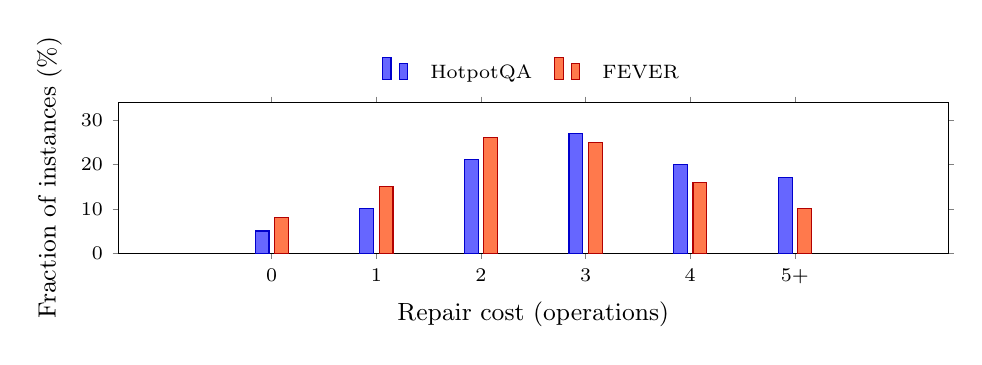
\begin{tikzpicture}
\begin{axis}[
  width=\columnwidth,
  height=3.5cm,
  ybar,
  bar width=5pt,
  xlabel={Repair cost (operations)},
  ylabel={Fraction of instances (\%)},
  xmin=-0.7, xmax=5.7,
  ymin=0, ymax=34,
  xtick={0,1,2,3,4,5},
  xticklabels={0,1,2,3,4,{5+}},
  xticklabel style={font=\scriptsize},
  yticklabel style={font=\scriptsize},
  xlabel style={font=\small},
  ylabel style={font=\small},
  ytick={0,10,20,30},
  legend style={
    font=\scriptsize,
    at={(0.5,1.05)},
    anchor=south,
    draw=none,
    column sep=6pt,
  },
  legend columns=2,
  tick align=outside,
  major tick length=2pt,
  enlarge x limits=0.12,
]
\addplot[fill=blue!60, draw=blue!80!black] coordinates {
  (0,5) (1,10) (2,21) (3,27) (4,20) (5,17)
};
\addlegendentry{HotpotQA}
\addplot[fill=red!50!orange!70, draw=red!70!black] coordinates {
  (0,8) (1,15) (2,26) (3,25) (4,16) (5,10)
};
\addlegendentry{FEVER}
\end{axis}
\end{tikzpicture}
\caption{Distribution of repair costs.  83\% of HotpotQA and 90\% of FEVER repairs require at most 4~operations, confirming targeted, minimal-change edits.}
\label{fig:cost-dist}
\end{figure}

Figure~\ref{fig:cost-dist} shows repair cost distributions concentrated at low values---means of \resultRepairCostHotpot{}/\resultRepairCostFEVER{} operations---confirming that most evidence updates require only local adjustments. The modal cost is 3 on HotpotQA, accounting for 27\% of instances, and 2 on FEVER at 26\%, reflecting FEVER's simpler reasoning chains.

A pilot human evaluation corroborates the automatic metrics; details appear in Appendix~\ref{app:human-eval}. Two annotators rated 75 HotpotQA instances in a blind design, preferring \textsc{Argus} in 68\% of comparisons vs.\ Self-Refine in 19\%, with inter-annotator agreement of $\kappa{=}0.62$; faithfulness ratings were 3.9 vs.\ 3.4 ($p{<}0.001$) and coherence ratings 4.1 vs.\ 3.8 ($p{=}0.012$). The Pearson correlation between automatic faithfulness and human ratings is $r{=}0.78$ ($p{<}0.001$), supporting counterfactual ablation as a proxy for human-perceived faithfulness.
